\documentclass[main.tex]{subfiles}
\begin{document}

\chapter{Kansruimten}
\label{cha:kansruimten}

\begin{de}
  Een \term{stochastisch experiment} is een experiment waarvan de uitkomst op voorhand onbekend is.
\end{de}

\begin{de}
  Een \term{Bernoulli experiment} is een experiment met maar twee mogelijke uitkomsten.
\end{de}
\section{Sigma algebra's}

\begin{de}
  Een \term{sigma algebra} of \term{$\sigma$-algebra} $\mathcal{A}$ is een verzameling $\mathcal{A}$ van deelverzamelingen van een \term{universum} $\Omega$ die voldoet aan de volgende drie axioma's.
  \begin{enumerate}
  \item $\Omega \in \mathcal{A}$
  \item $A\in \mathcal{A} \Rightarrow A^{C} \in \mathcal{A}$
  \item $(\forall n\in \mathbb{N}: A_{n} \in \mathcal{A}) \Rightarrow \bigcup_{n\in \mathbb{N}}A_{n} \in \mathcal{A}$
  \end{enumerate}
  De structuur $\Omega,\mathcal{A}$ wordt een \term{meetbare ruimte} genoemd en de verzamelingen in $\mathcal{A}$ noemen we \term{gebeurtenissen}.
\end{de}

\begin{st}
  $\emptyset \in \mathcal{A}$
\extra{bewijs}  
\end{st}

\begin{st}
  $(\forall n\in \{ 1,\dotsc,n \}: A_{n} \in \mathcal{A}) \Rightarrow \bigcup_{n\in \{1,\dotsc,n\}}A_{n} \in \mathcal{A}$
\extra{bewijs}  
\end{st}

\begin{st}
  $(\forall n\in \mathbb{N}: A_{n} \in \mathcal{A}) \Rightarrow \bigcap_{n\in \mathbb{N}}A_{n} \in \mathcal{A}$
\end{st}

\begin{st}
  $(\forall n\in \{ 1,\dotsc,n \}: A_{n} \in \mathcal{A}) \Rightarrow \bigcap_{n\in \{1,\dotsc,n\}}A_{n} \in \mathcal{A}$
\extra{bewijs}  
\end{st}

\begin{st}
  $\forall A,B \in \mathcal{A}: A \triangle B \in \mathcal{A}$
\end{st}

\begin{de}
  $\{ \emptyset, \Omega \}$ noemen we de \term{triviale $\sigma$-algebra}.
\end{de}
\begin{de}
  $\Omega,\{ \emptyset, \Omega \}$ noemen we de \term{triviale meetbare ruimte}.
\end{de}

\begin{de}
  De de machtsverzameling van een universum noemen we de \term{discrete $\sigma$-algebra}.
\end{de}


\section{Kansmaten}
\label{sec:kansmaten}

\begin{de}
  Zij $\mathcal{A}$ een kansruimten.
  Een \term{kansmaat} is een afbeelding $P:\ \mathcal{A} \rightarrow [0,1] \subset \mathbb{R}$ met de volgende eigenschappen.
  \begin{enumerate}
  \item $P(\Omega) = 1$
  \item $\forall A \in \mathcal{A}:\ P(A) \ge 0$
  \item Aftelbare additiviteit of $\sigma$-additiviteit: $\forall n\in \mathbb{N}, A_{n} \in \mathcal{A}, i \neq j:\ A_{i}\cap A_{j} = \emptyset$:
    \[ P\left( \bigcup_{n\in\mathbb{N}}A_{n} \right) = \sum_{n\in\mathbb{N}}P(A_{n}) \]
\extra{dit kan mooier geschreven,toch?}
  \end{enumerate}
  De structuur $\Omega,\mathcal{A},P$ noemen we een \term{kansruimte}.
\end{de} 

\begin{de}
  Zij $(A_{n})_{n}$ een rij verzamelingen, dan noemen we deze rij ...
  \begin{itemize}
  \item ... \term{stijgend} als $\forall n:\ A_{n}\subseteq A_{n+1}$ geldt: $A_{n}\uparrow$
  \item ... \term{dalend} als $\forall n:\ A_{n}\supseteq A_{n+1}$ geldt: $A_{n}\downarrow$
  \item ... \term{monotoon} als ze stijgend of dalend is.
  \end{itemize}
\end{de}

\begin{st}
  $A_{n} \uparrow \Rightarrow \lim_{n\rightarrow \infty}A_{n} = \bigcup_{n\in \mathbb{N}}^{\infty}A_{n}$.
\extra{bewijs}
\end{st}

\begin{st}
  $A_{n} \downarrow \Rightarrow \lim_{n\rightarrow \infty}A_{n} = \bigcap_{n\in \mathbb{N}}^{\infty}A_{n}$.
\extra{bewijs}
\end{st}

\begin{st}
  Zij $\Omega,\mathcal{A},P$ een kansruimte en $\{ A_{n} \mid n\in \{ 1,\dotsc,N\} \}$ $N$ paarsgewijze disjuncte gebeurtenissen.
  \[ P\left( \bigcup_{n=1}^{N}A_{n}\right) = \sum_{n=1}^{N}P(A_{n}) \]
\extra{bewijs}
\end{st}

\begin{st}
  Zij $\Omega,\mathcal{A},P$ een kansruimte.
  \[ \forall A \in \mathcal{A}:\ P(A^{C}) = 1 - P(A) \]
\extra{bewijs}
\end{st}

\begin{gev}
  $P(\emptyset) = 0$
\end{gev}

\begin{st}
  Zij $\Omega,\mathcal{A},P$ een kansruimte en $(A_{n})_{n}$ een monotone rij verzamelingen.
  \[ P\left( \lim_{n\rightarrow \infty}A_{n} \right) = \lim_{n\rightarrow \infty}P(A_{n}) \]
\extra{bewijs}
\end{st}

\begin{ei}
  Zij $\Omega,\mathcal{A},P$ een kansruimte.
  $\forall A,B \in \mathcal{A}:\ P(B) = P(B \cap A) + P(B \cap A^{C})$
\extra{bewijs}
\end{ei}

\begin{ei}
  Zij $\Omega,\mathcal{A},P$ een kansruimte.
  $\forall A,B \in \mathcal{A}:\ A \subseteq B \Rightarrow P(A) \le P(B)$
\extra{bewijs}
\end{ei}

\begin{ei}
  Zij $\Omega,\mathcal{A},P$ een kansruimte.
  $\forall A \in \mathcal{A}:\ P(A) \le 1$
\extra{bewijs}
\end{ei}

\begin{ei}
  Zij $\Omega,\mathcal{A},P$ een kansruimte.
  $\forall A,B \in \mathcal{A}:\ P(A \cup B) = P(A) + P(B) + P(A \cap B)$
\extra{bewijs}
\end{ei}

\section{Traditionele kansruimten}
\label{sec:trad-kansr}

\begin{de}
  De \term{uniforme kansmaat} is een kansmaat die enkel gedefini\"eerd is voor eindige verzamelingen.
  \[ P:\ \mathcal{A} \rightarrow [0,1] \subset \mathbb{R}:\ A \mapsto \frac{|A|}{|\Omega|} \]
\end{de}

\begin{de}
  De \term{discrete kansmaat} (?) is een kansmaat die enkel gedefini\"eerd is voor aftelbare verzamelingen.
  \[ P:\ \mathcal{A} \rightarrow [0,1] \subset \mathbb{R}:\ A \mapsto p_{i} \]
  Hier is het natuurlijk essentieel dat $\sum_{i}p_{i}=1$ geldt. 
\end{de}

\begin{de}
  Zij $\mathcal{C} \subseteq \Omega$ een collectie deelverzamelingen van een universum.
  De $\sigma$-algebra $\sigma(\mathcal{C})$ \term{voortgebracht door} $\mathcal{C}$ is de kleinste $\sigma$-algebra die $\mathcal{C}$ bevat.

  \begin{itemize}
  \item $\sigma(\mathcal{C}$ is een $\sigma$-algebra.
  \item $\mathcal{C} \subseteq \sigma(\mathcal{C})$
  \item Elke $\sigma$-algebra $\mathcal{A}$ met $\mathcal{C} \subseteq \mathcal{A}$ omvat $\sigma(\mathcal{C})$.
  \end{itemize}
\end{de}

\begin{st}
  De $\sigma$-algebra opgespannen door een collectie deelverzamelingen van een universum is uniek.
\extra{bewijs}
\end{st}

\begin{ei}
  Voor elke collectie deelverzamelingen $\mathcal{C} \subseteq \Omega$ bestaat $\sigma(C)$.
\TODO{bewijs p 13}
\end{ei}

\begin{de}
  De \term{Borel $\sigma$-algebra op $\mathbb{R}$} is de $\sigma$-algebra voortgebracht door $\mathcal{C}$:
  \[ \{ ]-\infty,a] \mid a \in \mathbb{R} \} \]  
\end{de}

\begin{st}
  Het \term{theorema van Vitali}\\
  Er bestaat geen uniforme kansverdeling op het interval $[0,1]$.
\zb
\end{st}

\section{Voorwaardelijke kans en onafhankelijkheid}
\label{sec:voorwaardelijke-kans-en-onafhankelijkheid}

\subsection{Voorwaardelijke kans}
\label{sec:voorwaardelijke-kans}

\begin{de}
  Zij $\Omega,\mathcal{A},P$ een kansruimte.
  De \term{voorwaardelijke kans} of \term{conditionele kans} van een gebeurtenis $A$ gegeven een gebeurtenis $B$ (met $P(B) \neq 0$) is $P(A|B)$.
  \[ P(A|B) = \frac{P(A\cap B)}{P(B)} \]
\end{de}

\begin{ei}
  $\forall A \in \mathcal{A}: P(A|A) = 1$
\extra{bewijs}
\end{ei}

\begin{ei}
  $\forall A \in \mathcal{A}: P(A|\Omega) = P(A)$
\extra{bewijs}
\end{ei}

\begin{st}
  Zij $\Omega,\mathcal{A},P$ een kansruimte en $B$ een gebeurtenis in $\mathcal{A}$ met kans groter dan nul.
  De functie $P_{B}$ is een kansmaat.
  \[ P_{B}:\ \mathcal{A} \rightarrow [0,1] \subset \mathbb{R}:\ A \mapsto P(A|B) \]
\end{st}

\subsection{Kettingregel}
\label{sec:kettingregel}

\begin{st}
  Zij $\Omega,\mathcal{A},P$ een kansruimte.
  Zij $\{ A_{1}, A_{2}, \dotsc, A_{k}\}$ meer dan \'e\'en gebeurtenis in $\mathcal{A}$.

  \[
  P\left(\bigcap_{i=1}^{k}A_{k}\right)
  = \prod_{i=1}^{k}P\left(A_{i}\mid\bigcap_{j=1}^{i-1}A_{j}\right)
  = P(A_{1})P(A_{2}|A_{1})P(A_{3}|A_{1}\cap A_{2}) \dotsb P(A_{k}|A_{1}\cap A_{2}\cap \dotsc \cap A_{k-1})
  \]
\extra{bewijs}
\end{st}

\subsection{Wet van de totale kans}
\label{sec:wet-van-de}

\begin{st}
  Zij $\Omega,\mathcal{A},P$ een kansruimte en $X$ een partitie van $\Omega$ waarin $\forall A \in X:\ P(A) > 0$ geldt.
  \[ \forall B \in A:\ P(B) = \sum_{A\in X}P(A)P(B|A) \]
  \extra{bewijs}
\end{st}

\subsection{Stelling van Bayes}
\label{sec:stelling-van-bayes}

\begin{ei}
  Zij $\Omega,\mathcal{A},P$ een kansruimte en $X$ een partitie van $\Omega$ waarin $\forall A \in X:\ P(A) > 0$ geldt.
  Zij $B$ een gebeurtenis in $\mathcal{A}$ met $P(B) > 0$.
  \[ \forall A\in X:\ P(A|B) = \frac{P(A)P(B|A)}{\sum_{C\in X}P(C)P(B|C)} \]
  \extra{bewijs}
\end{ei}

\subsection{Onafhankelijkheid}
\label{sec:onafhankelijkheid}
\begin{de}
  Zij $\Omega,\mathcal{A},P$ een kansruimte.
  We noemen twee gebeurtenissen $A$ en $B$ uit $\mathcal{A}$ \term{onafhankelijk} als het volgende geldt over hun kans:
  \[ P(A\cap B) = P(A) \cdot P(B) \]
\end{de}

\begin{de}
  Zij $\Omega,\mathcal{A},P$ een kansruimte en $A$ en $B$ twee afhankelijke gebeurtenissen uit $\mathcal{A}$ dan noemen we de afhankelijkheid ...
  \begin{itemize}
  \item ... \term{positieve afhankelijkheid} als $P(A \cap B) > P(A)P(B)$ geldt.
  \item ... \term{negatieve afhankelijkheid} als $P(A \cap B) < P(A)P(B)$ geldt.
  \end{itemize}
\end{de}

\begin{st}
  Zij $\Omega,\mathcal{A},P$ een kansruimte en $A$ en $B$ twee onafhankelijke gebeurtenissen uit $\mathcal{A}$.
  \[ P(A|B) = P(A) \]
  
  \extra{bewijs}
\end{st}

\begin{st}
  Zij $\Omega,\mathcal{A},P$ een kansruimte en $A$ en $B$ twee afhankelijke gebeurtenissen uit $\mathcal{A}$, dan zijn er twee mogelijkheden:
  \begin{itemize}
  \item $A$ en $B$ zijn positief afhankelijk: $P(A|B) > P(A)$.
  \item $A$ en $B$ zijn negatief afhankelijk: $P(A|B) < P(A)$.
  \end{itemize}
\end{st}

\begin{de}
  Een verzameling gebeurtenissen noemen we \term{paarsgewijs onafhankelijk} als elke twee gebeurtenissen onafhankelijk zijn.
\end{de}

\begin{de}
  Een eindige verzameling gebeurtenissen $X$ noemen we \term{onderling onafhankelijk} als het volgende geldt:
  \[ \forall Y\in \mathcal{P}(X):\ P\left( \bigcap_{A\in Y}A \right) = \prod_{A\in Y}P(A) \]
\end{de}

\begin{ei}
  Een onderling onafhankelijke verzameling gebeurtenissen is ook zeker paarsgewijs onafhankelijk.
\extra{bewijs}
\end{ei}

\begin{de}
  Een oneindige verzameling gebeurtenissen $X$ noemen we \term{onderling onafhankelijk} als elke eindige deelverzameling gebeurtenissen onderling onafhankelijk is.
\end{de}

\subsection{Systeembetrouwbaarheid}
\label{sec:syst}

\begin{figure}[H]
  \caption{Een serieel systeem}
  \centering
    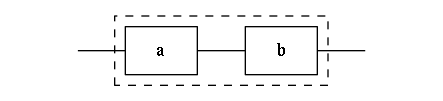
\includegraphics[width=0.5\textwidth]{assets/systeem-serieel.png}
\end{figure}

\begin{figure}[H]
  \caption{Een parallel systeem}
  \centering
    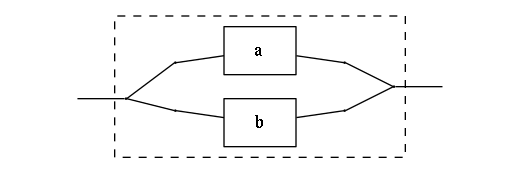
\includegraphics[width=0.5\textwidth]{assets/systeem-parallel.png}
\end{figure}

\begin{de}
  Een \term{serieel systeem} is een systeem met twee componenten dat werk als en slechts als beide componenten werken.
\end{de}

\begin{st}
  In een serieel systeem $S$ met componenten $A$ en $B$ met respectievelijke faalkansen $p_{A}$ en $p_{B}$ is de kans $p_{S}$ dat het systeem werkt als volgt.
  \[ p_{S} = p_{A} + p_{B} -p_{A}p_{B} \]
\TODO{bewijs p 23}
\end{st}

\begin{de}
  Een \term{parallel systeem} is een systeem met twee componenten dat werk als en slechts als \'e\'en van beide componenten werkt.
\end{de}

\begin{st}
  In een parallel systeem $S$ met componenten $A$ en $B$ met respectievelijke faalkansen $p_{A}$ en $p_{B}$ is de kans $p_{S}$ dat het systeem werkt als volgt.
  \[ p_{S} = p_{A}p_{B} \]
\TODO{bewijs p 24}
\end{st}


\end{document}

%%% Local Variables:
%%% mode: latex
%%% TeX-master: t
%%% End:
